\documentclass[12pt, a4paper]{article}

%% ── Geometry ────────────────────────────────────────────────────────────────
\usepackage[a4paper, top=2.5cm, bottom=2.5cm,
            left=2.8cm, right=2.8cm, headheight=15pt]{geometry}

%% ── Fonts & encoding ────────────────────────────────────────────────────────
\usepackage[T1]{fontenc}
\usepackage[utf8]{inputenc}
\usepackage{palatino}
\usepackage{mathpazo}
\usepackage{microtype}

%% ── Mathematics ─────────────────────────────────────────────────────────────
\usepackage{amsmath, amssymb, amsthm, mathtools}
\usepackage{cancel}

%% ── Graphics & colour ───────────────────────────────────────────────────────
\usepackage{xcolor}
\usepackage{tikz}
\usetikzlibrary{arrows.meta, positioning, calc,
                decorations.pathreplacing, backgrounds, patterns}
\usepackage{pgfplots}
\pgfplotsset{compat=1.15}

%% ── Tables ──────────────────────────────────────────────────────────────────
\usepackage{booktabs, array, colortbl, multirow, tabularx}
\renewcommand{\arraystretch}{1.45}

%% ── Lists ───────────────────────────────────────────────────────────────────
\usepackage{enumitem}
\setlist[itemize]{leftmargin=1.8em, itemsep=3pt, topsep=4pt}
\setlist[enumerate]{leftmargin=1.8em, itemsep=3pt, topsep=4pt}

%% ── Callout boxes ───────────────────────────────────────────────────────────
\usepackage[most]{tcolorbox}
\tcbuselibrary{skins, breakable, theorems}

%% ── Headers, footers, TOC, captions ────────────────────────────────────────
\usepackage{fancyhdr}
\usepackage{lastpage}
\usepackage{tocloft}
\usepackage{caption}
\usepackage{float}

%% ── Hyperlinks ──────────────────────────────────────────────────────────────
\usepackage[colorlinks=true, linkcolor=navy,
            urlcolor=navy, citecolor=navy]{hyperref}

%% ── Spacing ─────────────────────────────────────────────────────────────────
\usepackage{parskip}
\setlength{\parskip}{6pt}
\setlength{\parindent}{0pt}

%% ═══════════════════════════════════════════════════════════════════════════
%%  COLOUR PALETTE
%% ═══════════════════════════════════════════════════════════════════════════
\definecolor{navy}{RGB}{10, 40, 105}
\definecolor{navylight}{RGB}{230, 237, 252}
\definecolor{gold}{RGB}{175, 128, 8}
\definecolor{lightgold}{RGB}{254, 248, 218}
\definecolor{teal}{RGB}{8, 108, 98}
\definecolor{lightteal}{RGB}{222, 248, 243}
\definecolor{crimson}{RGB}{148, 18, 28}
\definecolor{lightcrimson}{RGB}{255, 234, 234}
\definecolor{purple}{RGB}{78, 28, 132}
\definecolor{lightpurple}{RGB}{244, 237, 255}
\definecolor{solgreen}{RGB}{8, 92, 48}
\definecolor{lightsol}{RGB}{225, 252, 236}
\definecolor{charcoal}{RGB}{36, 36, 36}
\definecolor{slate}{RGB}{72, 84, 100}
\definecolor{tabhead}{RGB}{10, 40, 105}
\definecolor{tabeven}{RGB}{230, 237, 252}
\definecolor{orange}{RGB}{195, 90, 10}
\definecolor{lightorange}{RGB}{255, 242, 225}

%% ═══════════════════════════════════════════════════════════════════════════
%%  TCOLORBOX ENVIRONMENTS
%% ═══════════════════════════════════════════════════════════════════════════

\newtcolorbox{defbox}[1]{breakable, enhanced,
  colback=navylight, colframe=navy, coltitle=white,
  fonttitle=\bfseries\sffamily, title={Definition\quad#1},
  arc=4pt, boxrule=1pt, left=8pt, right=8pt, top=6pt, bottom=6pt,
  attach boxed title to top left={yshift=-2mm, xshift=6mm},
  boxed title style={colback=navy, arc=3pt, boxrule=0pt}}

\newtcolorbox{thmbox}[1]{breakable, enhanced,
  colback=lightteal, colframe=teal, coltitle=white,
  fonttitle=\bfseries\sffamily, title={Theorem\quad#1},
  arc=4pt, boxrule=1pt, left=8pt, right=8pt, top=6pt, bottom=6pt,
  attach boxed title to top left={yshift=-2mm, xshift=6mm},
  boxed title style={colback=teal, arc=3pt, boxrule=0pt}}

\newtcolorbox{propbox}[1]{breakable, enhanced,
  colback=lightteal, colframe=teal, coltitle=white,
  fonttitle=\bfseries\sffamily, title={Proposition\quad#1},
  arc=4pt, boxrule=1pt, left=8pt, right=8pt, top=6pt, bottom=6pt,
  attach boxed title to top left={yshift=-2mm, xshift=6mm},
  boxed title style={colback=teal, arc=3pt, boxrule=0pt}}

\newtcolorbox{keybox}[1]{breakable, enhanced,
  colback=lightgold, colframe=gold, coltitle=white,
  fonttitle=\bfseries\sffamily, title={#1},
  arc=4pt, boxrule=1pt, left=8pt, right=8pt, top=6pt, bottom=6pt,
  attach boxed title to top left={yshift=-2mm, xshift=6mm},
  boxed title style={colback=gold, arc=3pt, boxrule=0pt}}

\newtcolorbox{exbox}[1]{breakable, enhanced,
  colback=lightpurple, colframe=purple, coltitle=white,
  fonttitle=\bfseries\sffamily, title={Worked Example\quad#1},
  arc=4pt, boxrule=1pt, left=8pt, right=8pt, top=6pt, bottom=6pt,
  attach boxed title to top left={yshift=-2mm, xshift=6mm},
  boxed title style={colback=purple, arc=3pt, boxrule=0pt}}

\newtcolorbox{warnbox}[1]{breakable, enhanced,
  colback=lightcrimson, colframe=crimson, coltitle=white,
  fonttitle=\bfseries\sffamily, title={#1},
  arc=4pt, boxrule=1pt, left=8pt, right=8pt, top=6pt, bottom=6pt,
  attach boxed title to top left={yshift=-2mm, xshift=6mm},
  boxed title style={colback=crimson, arc=3pt, boxrule=0pt}}

\newtcolorbox{notebox}[1]{breakable, enhanced,
  colback=lightorange, colframe=orange, coltitle=white,
  fonttitle=\bfseries\sffamily, title={#1},
  arc=4pt, boxrule=1pt, left=8pt, right=8pt, top=6pt, bottom=6pt,
  attach boxed title to top left={yshift=-2mm, xshift=6mm},
  boxed title style={colback=orange, arc=3pt, boxrule=0pt}}

\newtcolorbox{solbox}{breakable, enhanced,
  colback=lightsol, colframe=solgreen, coltitle=white,
  fonttitle=\bfseries\sffamily, title={Solution},
  arc=4pt, boxrule=1pt, left=8pt, right=8pt, top=6pt, bottom=6pt,
  attach boxed title to top left={yshift=-2mm, xshift=6mm},
  boxed title style={colback=solgreen, arc=3pt, boxrule=0pt}}

%% ── Theorem-style environments ──────────────────────────────────────────────
\theoremstyle{definition}
\newtheorem{remark}{Remark}[section]

%% ═══════════════════════════════════════════════════════════════════════════
%%  MATHS MACROS
%% ═══════════════════════════════════════════════════════════════════════════
\newcommand{\R}{\mathbb{R}}
\newcommand{\N}{\mathbb{N}}
\newcommand{\bx}{\mathbf{x}}
\newcommand{\bz}{\mathbf{0}}
\newcommand{\bH}{\mathbf{H}}
\newcommand{\bJ}{\mathbf{J}}
\newcommand{\ddd}[2]{\dfrac{d#1}{d#2}}
\newcommand{\pp}[2]{\dfrac{\partial #1}{\partial #2}}
\newcommand{\ppp}[2]{\dfrac{\partial^2 #1}{\partial #2^2}}
\newcommand{\ppmix}[3]{\dfrac{\partial^2 #1}{\partial #2\,\partial #3}}
\newcommand{\eval}[2]{\left.#1\right|_{#2}}
\newcommand{\abs}[1]{\left|#1\right|}
\newcommand{\norm}[1]{\left\|#1\right\|}
\newcommand{\st}{\;\text{s.t.}\;}
\newcommand{\grad}{\nabla}
\DeclareMathOperator{\tr}{tr}
\DeclareMathOperator{\rank}{rank}
\DeclareMathOperator{\sgn}{sgn}
\DeclareMathOperator{\argmax}{arg\,max}
\DeclareMathOperator{\argmin}{arg\,min}

%% ═══════════════════════════════════════════════════════════════════════════
%%  PAGE STYLE
%% ═══════════════════════════════════════════════════════════════════════════
\pagestyle{fancy}
\fancyhf{}
\fancyhead[L]{\textcolor{navy}{\textbf{ECON 320}}
  \textcolor{slate}{ --- Optimisation of Multi-Variable Functions}}

\fancyfoot[C]{\textcolor{slate}{\small Page \thepage\ of \pageref{LastPage}}}
\renewcommand{\headrulewidth}{1.2pt}
\renewcommand{\headrule}{%
  \hbox to\headwidth{\color{navy}\leaders\hrule height\headrulewidth\hfill}}
\renewcommand{\footrulewidth}{0.4pt}

\renewcommand{\cftsecfont}{\bfseries\color{navy}}
\renewcommand{\cftsecpagefont}{\bfseries\color{navy}}
\renewcommand{\cftsubsecfont}{\color{charcoal}}
\setlength{\cftbeforesecskip}{4pt}

%% ═══════════════════════════════════════════════════════════════════════════
\begin{document}
%% ═══════════════════════════════════════════════════════════════════════════

%% ── COVER ───────────────────────────────────────────────────────────────────
\thispagestyle{empty}
\begin{tikzpicture}[remember picture, overlay]
  \fill[navy]  (current page.north west)
    rectangle ([yshift=-6.2cm] current page.north east);
  \fill[gold]  ([yshift=-6.2cm] current page.north west)
    rectangle ([yshift=-6.65cm] current page.north east);
\end{tikzpicture}

\vspace*{-1.7cm}
\begin{center}
  {\color{white}\large\bfseries\sffamily ECON 320 --- LECTURE NOTES}\\[10pt]
  {\color{white}\Huge\bfseries Optimisation of}\\[6pt]
  {\color{white}\Huge\bfseries Multi-Variable Functions}\\[10pt]
  {\color{gold}\large\itshape
    Chiang \& Wainwright (2005) Ch.\ 11--12\quad|\quad
    Hoy et al.\ (2011)\quad|\quad Simon \& Blume (1994)}
\end{center}

\vspace{3.8cm}
\begin{center}
\begin{tabular}{r l}
  \textbf{\textcolor{navy}{Course}}
    & ECON 320: Mathematical Economics III \\[3pt]
  \textbf{\textcolor{navy}{Primary Text}}
    & A.\ C.\ Chiang \& K.\ Wainwright,
      \textit{Fundamental Methods of Mathematical Economics},\\
    & 4th ed., McGraw-Hill, 2005. \\[3pt]
  \textbf{\textcolor{navy}{Supplementary}}
    & Hoy, Livernois, McKenna, Rees \& Stengos,
      \textit{Mathematics for Economics},\\
    & 3rd ed., MIT Press, 2011. \\[2pt]
    & Simon \& Blume, \textit{Mathematics for Economists},
      Norton, 1994. \\[3pt]
  \textbf{\textcolor{navy}{Topics}}
    & Unconstrained optimisation, first- and second-order conditions,\\
    & Hessian matrix, definiteness, global optima, concavity/convexity,\\
    & constrained optimisation, Lagrange multipliers, bordered Hessian,\\
    & envelope theorem, comparative statics. \\[3pt]
  \textbf{\textcolor{navy}{Date}} & May 2026 \\
\end{tabular}
\end{center}

\newpage
\tableofcontents
\newpage

%% ═══════════════════════════════════════════════════════════════════════════
\section{From One Variable to Many: The Setting}
%% ═══════════════════════════════════════════════════════════════════════════

Most economic problems involve choosing \emph{several} variables
simultaneously. A consumer chooses a bundle $(x_1,\ldots,x_n)$; a firm
chooses inputs $(K, L)$ and output $Q$; a central planner allocates resources
across sectors. Single-variable analysis is an essential stepping stone, but
the real engine of economic theory is multi-variable optimisation.

The essential new challenges in moving from one to many variables are:
\begin{itemize}
  \item The gradient replaces the derivative, and the condition $\nabla f = \bz$
        gives a \emph{system} of equations.
  \item The second-order condition involves not just a single number $f''(x^*)$
        but a \emph{matrix} of second derivatives --- the \textbf{Hessian}.
  \item The sign properties of a matrix (positive/negative definiteness)
        generalise the sign of $f''$.
  \item Constrained optimisation introduces the method of \textbf{Lagrange
        multipliers} and the \textbf{bordered Hessian}.
\end{itemize}

Throughout, we work in $\R^n$ and write vectors as
$\bx = (x_1, x_2, \ldots, x_n)^\top$. Objective functions are
$f: D \subseteq \R^n \to \R$.

%% ═══════════════════════════════════════════════════════════════════════════
\section{Unconstrained Optimisation: First-Order Conditions}
%% ═══════════════════════════════════════════════════════════════════════════

\subsection{The Gradient and Critical Points}

\begin{defbox}{Gradient Vector}
The \textbf{gradient} of $f: \R^n \to \R$ at $\bx$ is the vector of
first-order partial derivatives:
\[
  \nabla f(\bx)
  = \begin{pmatrix}
      f_{x_1}(\bx) \\ f_{x_2}(\bx) \\ \vdots \\ f_{x_n}(\bx)
    \end{pmatrix}
  = \begin{pmatrix}
      \partial f/\partial x_1 \\
      \partial f/\partial x_2 \\
      \vdots \\
      \partial f/\partial x_n
    \end{pmatrix}
\]
The gradient points in the direction of steepest ascent of $f$ at $\bx$.
\end{defbox}

\begin{thmbox}{First-Order Necessary Condition (FOC)}
Let $f: D \subseteq \R^n \to \R$ be differentiable. A \textbf{necessary}
condition for $\bx^*$ to be a local maximum or local minimum of $f$ at an
interior point of $D$ is:
\[
  \boxed{\nabla f(\bx^*) = \bz}
  \qquad\Longleftrightarrow\qquad
  \pp{f}{x_j}(\bx^*) = 0 \quad \text{for all } j = 1, \ldots, n
\]
A point satisfying this condition is called a \textbf{critical point}
(or \textbf{stationary point}) of $f$.
\emph{(Chiang \& Wainwright, p.\ 318; Simon \& Blume, Ch.\ 17)}
\end{thmbox}

\begin{keybox}{Economic Interpretation of the Multi-Variable FOC}
Each equation $f_{x_j}(\bx^*) = 0$ says the \emph{marginal contribution}
of variable $j$ to the objective is zero at the optimum. In:
\begin{itemize}
  \item \textbf{Profit maximisation}: $\partial\pi/\partial K = 0$ and
        $\partial\pi/\partial L = 0$ mean the value marginal product of
        each input equals its price.
  \item \textbf{Utility maximisation} (unconstrained): marginal utility of
        each good is zero --- the satiation point.
  \item \textbf{Multiproduct firm}: $\partial\pi/\partial Q_i = 0$ for each
        product $i$ means $\text{MR}_i = \text{MC}_i$.
\end{itemize}
\end{keybox}

\begin{exbox}{Finding Critical Points --- Two Variables}
Find all critical points of $f(x, y) = x^3 + y^3 - 3x - 3y + 8$.

\textbf{Step 1 --- Compute partial derivatives:}
\[
  f_x = 3x^2 - 3 = 3(x^2-1), \qquad f_y = 3y^2 - 3 = 3(y^2-1)
\]

\textbf{Step 2 --- Set equal to zero and solve:}
\[
  f_x = 0 \Rightarrow x = \pm 1, \qquad f_y = 0 \Rightarrow y = \pm 1
\]

\textbf{Step 3 --- Enumerate all critical points:}
$(1,1)$, $(1,-1)$, $(-1,1)$, $(-1,-1)$ --- four critical points.

\textbf{Critical values:}
$f(1,1) = 1+1-3-3+8 = 4$,\quad
$f(1,-1) = 1-1-3+3+8 = 8$,\quad
$f(-1,1) = -1+1+3-3+8 = 8$,\quad
$f(-1,-1) = -1-1+3+3+8 = 12$.

To classify these points, we need the second-order conditions.
\end{exbox}
\newpage
%% ═══════════════════════════════════════════════════════════════════════════
\section{The Hessian Matrix and Second-Order Conditions}
%% ═══════════════════════════════════════════════════════════════════════════

\subsection{The Hessian Matrix}

\begin{defbox}{Hessian Matrix}
The \textbf{Hessian matrix} of $f: \R^n \to \R$ (assumed twice
continuously differentiable) at $\bx$ is the $n \times n$ symmetric matrix
of all second-order partial derivatives:
\[
  \bH(\bx) = \begin{pmatrix}
    f_{x_1 x_1} & f_{x_1 x_2} & \cdots & f_{x_1 x_n} \\
    f_{x_2 x_1} & f_{x_2 x_2} & \cdots & f_{x_2 x_n} \\
    \vdots       & \vdots       & \ddots & \vdots \\
    f_{x_n x_1} & f_{x_n x_2} & \cdots & f_{x_n x_n}
  \end{pmatrix}
\]
By Young's Theorem (continuity of mixed partials),
$f_{x_i x_j} = f_{x_j x_i}$, so $\bH$ is symmetric.

For $n=2$:
\[
  \bH = \begin{pmatrix} f_{xx} & f_{xy} \\ f_{xy} & f_{yy} \end{pmatrix}
\]
\end{defbox}

\begin{keybox}{The Hessian as a Multi-Variable Second Derivative}
In single-variable analysis, the sign of $f''(x^*)$ determines whether
$x^*$ is a max or min. In multi-variable analysis, the \emph{definiteness}
of $\bH(\bx^*)$ plays exactly the same role:
\begin{itemize}
  \item $\bH$ \textbf{negative definite} $\leftrightarrow$ $f$ is locally
        concave $\leftrightarrow$ local maximum.
  \item $\bH$ \textbf{positive definite} $\leftrightarrow$ $f$ is locally
        convex $\leftrightarrow$ local minimum.
\end{itemize}
\end{keybox}

\subsection{Quadratic Forms and Definiteness}

\begin{defbox}{Quadratic Form and Definiteness}
A \textbf{quadratic form} associated with a symmetric $n \times n$ matrix
$\bH$ is $Q(\mathbf{d}) = \mathbf{d}^\top \bH\, \mathbf{d}$ for
$\mathbf{d} \in \R^n$.

The matrix $\bH$ is:
\begin{itemize}
  \item \textbf{Positive definite (PD)}: $Q(\mathbf{d}) > 0$ for all
        $\mathbf{d} \neq \bz$.
  \item \textbf{Negative definite (ND)}: $Q(\mathbf{d}) < 0$ for all
        $\mathbf{d} \neq \bz$.
  \item \textbf{Positive semi-definite (PSD)}: $Q(\mathbf{d}) \geq 0$ for
        all $\mathbf{d}$.
  \item \textbf{Negative semi-definite (NSD)}: $Q(\mathbf{d}) \leq 0$ for
        all $\mathbf{d}$.
  \item \textbf{Indefinite}: $Q$ takes both positive and negative values.
\end{itemize}
\end{defbox}

\subsection{Checking Definiteness: Leading Principal Minors}

\begin{defbox}{Leading Principal Minors}
The \textbf{$k$-th leading principal minor} of a matrix $\bH$, denoted
$|\bH_k|$ or $D_k$, is the determinant of the top-left $k \times k$
submatrix:
\[
  D_1 = |f_{x_1 x_1}|, \quad
  D_2 = \begin{vmatrix} f_{x_1 x_1} & f_{x_1 x_2} \\ f_{x_2 x_1} & f_{x_2 x_2} \end{vmatrix}, \quad
  \ldots, \quad
  D_n = |\bH|
\]
\end{defbox}

\begin{thmbox}{Definiteness via Leading Principal Minors}
Let $\bH$ be a real symmetric $n \times n$ matrix with leading principal
minors $D_1, D_2, \ldots, D_n$.
\begin{enumerate}
  \item $\bH$ is \textbf{positive definite} if and only if
        $D_k > 0$ for all $k = 1, \ldots, n$:
        \[
          D_1 > 0,\quad D_2 > 0,\quad \ldots,\quad D_n > 0
        \]
  \item $\bH$ is \textbf{negative definite} if and only if
        the leading principal minors alternate in sign starting negative:
        \[
          D_1 < 0,\quad D_2 > 0,\quad D_3 < 0,\quad \ldots,\quad
          (-1)^k D_k > 0 \text{ for all } k
        \]
  \item If neither condition holds and $D_n \neq 0$: $\bH$ is
        \textbf{indefinite}.
  \item If $D_n = 0$: $\bH$ is \textbf{singular} (semi-definite or
        indefinite; further analysis required).
\end{enumerate}
\emph{(Chiang \& Wainwright, p.\ 322; Simon \& Blume, Theorem~16.3;
Hoy et al., p.\ 396)}
\end{thmbox}

\begin{exbox}{Checking Definiteness for $n=2$}
For $n=2$ with $\bH = \begin{pmatrix} a & b \\ b & d \end{pmatrix}$:

$D_1 = a$, \quad $D_2 = ad - b^2$.

\begin{center}
\begin{tabular}{lll}
  \toprule
  \rowcolor{tabhead}
  \color{white}Condition & \color{white}Definiteness & \color{white}Interpretation \\
  \midrule
  $a > 0$ and $ad - b^2 > 0$
    & \textbf{Positive Definite} & Local minimum \\
  \rowcolor{tabeven}
  $a < 0$ and $ad - b^2 > 0$
    & \textbf{Negative Definite} & Local maximum \\
  $ad - b^2 < 0$
    & \textbf{Indefinite} & Saddle point \\
  \rowcolor{tabeven}
  $ad - b^2 = 0$
    & Singular (semi-definite) & Inconclusive \\
  \bottomrule
\end{tabular}
\end{center}

Note: For ND with $n=2$, the condition $a < 0$ and $ad-b^2 > 0$ follows
from the sign-alternating rule: $D_1 = a < 0$ and $D_2 = ad-b^2 > 0$.
\end{exbox}

\subsection{Second-Order Sufficient Conditions}

\begin{thmbox}{Second-Order Sufficient Conditions (SOC)}
Let $f: \R^n \to \R$ be twice continuously differentiable and suppose
$\nabla f(\bx^*) = \bz$ (FOC satisfied). Then:
\begin{itemize}
  \item If $\bH(\bx^*)$ is \textbf{negative definite}: $\bx^*$ is a
        \textbf{strict local maximum}.
  \item If $\bH(\bx^*)$ is \textbf{positive definite}: $\bx^*$ is a
        \textbf{strict local minimum}.
  \item If $\bH(\bx^*)$ is \textbf{indefinite}: $\bx^*$ is a
        \textbf{saddle point} (neither max nor min).
  \item If $\bH(\bx^*)$ is \textbf{semi-definite}: \emph{inconclusive}
        --- higher-order analysis required.
\end{itemize}
\emph{(Chiang \& Wainwright, p.\ 319; Hoy et al., p.\ 393)}
\end{thmbox}

\begin{keybox}{Taylor Expansion Justification}
The second-order Taylor expansion of $f$ around $\bx^*$ gives:
\[
  f(\bx^* + \mathbf{d}) - f(\bx^*)
  \approx \underbrace{\nabla f(\bx^*)^\top \mathbf{d}}_{=\,0\text{ by FOC}}
  + \frac{1}{2}\mathbf{d}^\top \bH(\bx^*)\mathbf{d}
  = \frac{1}{2}\mathbf{d}^\top \bH(\bx^*)\mathbf{d}
\]
for small $\mathbf{d}$. If $\bH(\bx^*)$ is ND, then
$\mathbf{d}^\top \bH(\bx^*)\mathbf{d} < 0$ for all $\mathbf{d} \neq \bz$,
so $f(\bx^*+\mathbf{d}) < f(\bx^*)$ --- confirming a local maximum.
\end{keybox}

\begin{exbox}{Full FOC and SOC Analysis --- Two Variables}
Find and classify all critical points of
$f(x,y) = x^3 + y^3 - 3x - 3y + 8$ (continued from Section~2).

\textbf{Hessian:}
\[
  f_{xx} = 6x, \quad f_{xy} = 0, \quad f_{yy} = 6y
  \qquad\Rightarrow\qquad
  \bH(x,y) = \begin{pmatrix} 6x & 0 \\ 0 & 6y \end{pmatrix}
\]

\textbf{Classification at each critical point:}
\smallskip

\begin{center}
\begin{tabular}{cccccl}
  \toprule
  \rowcolor{tabhead}
  \color{white}Point & \color{white}$D_1 = 6x$ & \color{white}$D_2 = 36xy$
  & \color{white}$f(\bx^*)$ & \color{white}Type \\
  \midrule
  $(1,1)$   & $6>0$  & $36>0$   & $4$  & \textbf{Local min} (PD) \\
  \rowcolor{tabeven}
  $(1,-1)$  & $6>0$  & $-36<0$  & $8$  & \textbf{Saddle point} (Indefinite) \\
  $(-1,1)$  & $-6<0$ & $-36<0$  & $8$  & \textbf{Saddle point} (Indefinite) \\
  \rowcolor{tabeven}
  $(-1,-1)$ & $-6<0$ & $36>0$   & $12$ & \textbf{Local max} (ND) \\
  \bottomrule
\end{tabular}
\end{center}

\medskip
At $(-1,-1)$: $D_1=-6<0$ and $D_2=36>0$ confirms negative definiteness
(sign pattern $-,+$). \checkmark

At $(1,-1)$: $D_2=-36<0$ implies indefiniteness (saddle point). \checkmark
\end{exbox}

\subsection{Saddle Points}

\begin{defbox}{Saddle Point}
A critical point $\bx^*$ is a \textbf{saddle point} if $\nabla f(\bx^*)=\bz$
but $\bx^*$ is neither a local maximum nor a local minimum. This occurs when
$\bH(\bx^*)$ is indefinite: the function increases in some directions from
$\bx^*$ and decreases in others.
\end{defbox}

\begin{center}
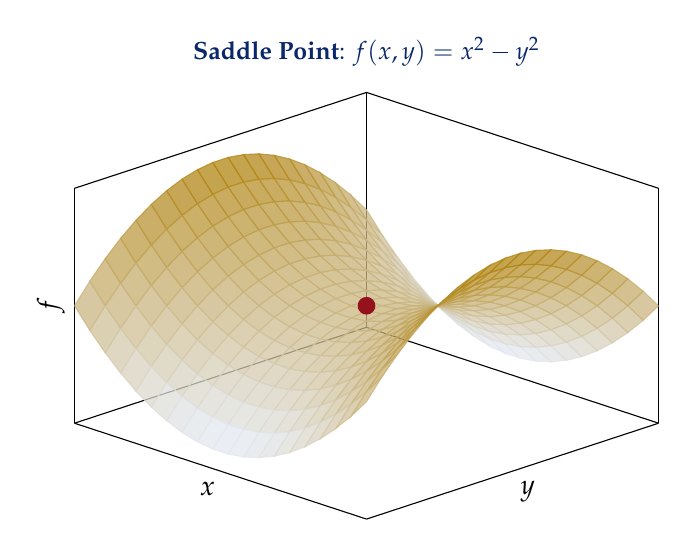
\begin{tikzpicture}
\begin{axis}[
  width=9cm, height=7cm,
  view={45}{30},
  xlabel={$x$}, ylabel={$y$}, zlabel={$f$},
  title={\small\textbf{Saddle Point}: $f(x,y)=x^2-y^2$},
  title style={color=navy},
  xtick=\empty, ytick=\empty, ztick=\empty,
  colormap={navygold}{color=(navylight) color=(gold)},
]
  \addplot3[surf, opacity=0.75, samples=20,
    domain=-1.5:1.5, domain y=-1.5:1.5,
    shader=flat]
    {x^2 - y^2};
  \addplot3[only marks, mark=*, mark size=3pt, crimson]
    coordinates {(0,0,0)};
\end{axis}
\end{tikzpicture}
\captionof*{figure}{\small $f(x,y)=x^2-y^2$: maximum along the $y$-axis,
minimum along the $x$-axis at the origin --- a saddle point.
$\bH = \begin{pmatrix}2&0\\0&-2\end{pmatrix}$: indefinite.}
\end{center}

%% ═══════════════════════════════════════════════════════════════════════════
\section{Global Optima: Concavity and Convexity in $\R^n$}
%% ═══════════════════════════════════════════════════════════════════════════

\subsection{Multi-Variable Concavity and Convexity}

\begin{defbox}{Concave and Convex Functions on $\R^n$}
A function $f: C \to \R$ on a convex set $C \subseteq \R^n$ is:
\begin{itemize}
  \item \textbf{Concave}: $f(\lambda\bx + (1-\lambda)\mathbf{y}) \geq
        \lambda f(\bx) + (1-\lambda)f(\mathbf{y})$ for all
        $\bx, \mathbf{y} \in C$ and $\lambda \in [0,1]$.
  \item \textbf{Convex}: $f(\lambda\bx + (1-\lambda)\mathbf{y}) \leq
        \lambda f(\bx) + (1-\lambda)f(\mathbf{y})$ for all
        $\bx, \mathbf{y} \in C$ and $\lambda \in [0,1]$.
  \item \textbf{Strictly concave/convex}: strict inequalities for
        $\lambda \in (0,1)$ and $\bx \neq \mathbf{y}$.
\end{itemize}
\end{defbox}

\begin{thmbox}{Hessian Characterisation of Global Concavity/Convexity}
If $f$ is twice continuously differentiable on a convex open set $C$:
\begin{itemize}
  \item $f$ is \textbf{concave} on $C$ $\iff$
        $\bH(\bx)$ is \textbf{negative semi-definite} for all $\bx \in C$.
  \item $f$ is \textbf{convex} on $C$ $\iff$
        $\bH(\bx)$ is \textbf{positive semi-definite} for all $\bx \in C$.
  \item $\bH(\bx)$ \textbf{negative definite} for all $\bx \in C$
        $\Rightarrow$ $f$ is \textbf{strictly concave}.
  \item $\bH(\bx)$ \textbf{positive definite} for all $\bx \in C$
        $\Rightarrow$ $f$ is \textbf{strictly convex}.
\end{itemize}
\emph{(Chiang \& Wainwright, p.\ 327; Simon \& Blume, Theorem~21.9)}
\end{thmbox}

\begin{thmbox}{Global Optimality from Concavity/Convexity}
\begin{itemize}
  \item If $f$ is \textbf{concave} on $C$ and $\nabla f(\bx^*) = \bz$
        for interior $\bx^* \in C$:
        $\bx^*$ is a \textbf{global maximum} of $f$ on $C$.
  \item If $f$ is \textbf{convex} on $C$ and $\nabla f(\bx^*) = \bz$
        for interior $\bx^* \in C$:
        $\bx^*$ is a \textbf{global minimum} of $f$ on $C$.
  \item Under \emph{strict} concavity/convexity, the global optimum is
        \textbf{unique}.
\end{itemize}
\end{thmbox}

\begin{exbox}{Multiproduct Monopoly --- Global Maximum}
A monopolist produces two goods with inverse demands
$P_1 = 40 - 2Q_1$ and $P_2 = 30 - Q_2$,
and joint cost $C = Q_1^2 + Q_1 Q_2 + Q_2^2$.

\textbf{Profit:}
\[
  \pi(Q_1, Q_2)
  = P_1 Q_1 + P_2 Q_2 - C
  = (40-2Q_1)Q_1 + (30-Q_2)Q_2 - Q_1^2 - Q_1 Q_2 - Q_2^2
\]
\[
  = 40Q_1 - 2Q_1^2 + 30Q_2 - Q_2^2 - Q_1^2 - Q_1 Q_2 - Q_2^2
  = 40Q_1 + 30Q_2 - 3Q_1^2 - Q_1 Q_2 - 2Q_2^2
\]

\textbf{FOC:}
\[
  \pi_1 = 40 - 6Q_1 - Q_2 = 0 \quad (1)
\]
\[
  \pi_2 = 30 - Q_1 - 4Q_2 = 0 \quad (2)
\]

From (2): $Q_1 = 30 - 4Q_2$. Substitute into (1):
$40 - 6(30-4Q_2) - Q_2 = 0$
$\Rightarrow 40 - 180 + 24Q_2 - Q_2 = 0$
$\Rightarrow 23Q_2 = 140 \Rightarrow Q_2^* = 140/23 \approx 6.09$.

$Q_1^* = 30 - 4(140/23) = 30 - 560/23 = (690-560)/23 = 130/23 \approx 5.65$.

\textbf{SOC --- Hessian:}
\[
  \bH = \begin{pmatrix} -6 & -1 \\ -1 & -4 \end{pmatrix}
\]
$D_1 = -6 < 0$, \quad $D_2 = (-6)(-4) - (-1)^2 = 24-1 = 23 > 0$.

Sign pattern: $(-, +)$ --- \textbf{negative definite}. Since $\bH$ is ND
\emph{everywhere} (it is constant), $\pi$ is strictly concave globally.
The critical point $(Q_1^*, Q_2^*)$ is the \textbf{unique global maximum}. \checkmark

\textbf{Optimal prices and profit:}
$P_1^* = 40-2(130/23) = (920-260)/23 = 660/23 \approx 28.70$
$P_2^* = 30-140/23 = (690-140)/23 = 550/23 \approx 23.91$
$\pi^* = (660/23)(130/23) + (550/23)(140/23) - \ldots \approx 232$ (verify numerically).
\end{exbox}

%% ═══════════════════════════════════════════════════════════════════════════
\section{Constrained Optimisation: Equality Constraints}
%% ═══════════════════════════════════════════════════════════════════════════

\subsection{The Problem and Its Geometry}

Most economic optimisation problems involve \emph{constraints}. A consumer
maximises utility \emph{subject to} a budget constraint; a firm minimises
cost \emph{subject to} a production target.

The standard problem with one equality constraint is:
\[
  \max_{\bx} f(\bx) \quad \text{subject to} \quad g(\bx) = c
\]
where $f: \R^n \to \R$ is the objective and $g(\bx) = c$ defines the
constraint set.

\textbf{Geometric insight.} At the constrained optimum, the level curves of
$f$ (indifference curves or iso-profit curves) are \emph{tangent} to the
constraint curve $g(\bx)=c$. Tangency means the gradients are parallel:
$\nabla f = \lambda \nabla g$ for some scalar $\lambda$.

\subsection{The Lagrangian Method}

\begin{defbox}{Lagrangian Function}
The \textbf{Lagrangian} associated with the constrained problem
$\max f(\bx) \st g(\bx) = c$ is:
\[
  \mathcal{L}(\bx, \lambda)
  = f(\bx) - \lambda[g(\bx) - c]
  = f(\bx) + \lambda[c - g(\bx)]
\]
where $\lambda \in \R$ is the \textbf{Lagrange multiplier}.
\end{defbox}

\begin{thmbox}{Lagrange's Theorem (First-Order Necessary Conditions)}
Let $f$ and $g$ be continuously differentiable. If $\bx^*$ is a constrained
local optimum of $f$ on $\{g(\bx)=c\}$, and if the \emph{constraint
qualification} $\nabla g(\bx^*) \neq \bz$ holds, then there exists a scalar
$\lambda^*$ such that:
\[
  \nabla f(\bx^*) = \lambda^* \nabla g(\bx^*)
\]
Equivalently, $\bx^*$ and $\lambda^*$ satisfy the
\textbf{Lagrange conditions}:
\begin{align}
  \mathcal{L}_{x_j} = f_{x_j}(\bx^*) - \lambda^* g_{x_j}(\bx^*) &= 0,
  \quad j = 1,\ldots,n \label{eq:L_x}\\
  \mathcal{L}_\lambda = g(\bx^*) - c &= 0 \label{eq:L_lam}
\end{align}
This gives $n+1$ equations in $n+1$ unknowns $(x_1^*, \ldots, x_n^*, \lambda^*)$.
\emph{(Chiang \& Wainwright, p.\ 359; Hoy et al., p.\ 430; Simon \& Blume, Theorem~18.2)}
\end{thmbox}

\begin{keybox}{Interpretation of the Lagrange Multiplier $\lambda^*$}
$\lambda^*$ measures the \textbf{shadow price} of the constraint:
\[
  \lambda^* = \ddd{f^*(c)}{c}
  \quad\text{where } f^*(c) = \max_{\bx\,:\,g(\bx)=c} f(\bx)
\]
It gives the marginal change in the \emph{optimal value} of the objective
when the constraint level $c$ is relaxed by one unit. In:
\begin{itemize}
  \item \textbf{Consumer theory}: $\lambda^*$ is the marginal utility of
        income (how much utility rises for a \$1 increase in budget).
  \item \textbf{Firm's cost minimisation}: $\lambda^*$ is the marginal
        cost of increasing the output target.
  \item \textbf{Resource allocation}: $\lambda^*$ is the marginal value
        of relaxing the resource constraint.
\end{itemize}
\end{keybox}
\newpage
\begin{exbox}{Utility Maximisation --- Standard Consumer Problem}
Maximise $U(x_1, x_2) = x_1^{1/2} x_2^{1/2}$ subject to
$p_1 x_1 + p_2 x_2 = m$ (budget constraint), with $p_1, p_2, m > 0$.

\textbf{Lagrangian:}
\[
  \mathcal{L} = x_1^{1/2}x_2^{1/2} - \lambda(p_1 x_1 + p_2 x_2 - m)
\]

\textbf{Lagrange conditions:}
\[
  \mathcal{L}_{x_1} = \frac{1}{2}x_1^{-1/2}x_2^{1/2} - \lambda p_1 = 0
  \quad\Rightarrow\quad
  \frac{1}{2}\cdot\frac{x_2^{1/2}}{x_1^{1/2}} = \lambda p_1 \tag{1}
\]
\[
  \mathcal{L}_{x_2} = \frac{1}{2}x_1^{1/2}x_2^{-1/2} - \lambda p_2 = 0
  \quad\Rightarrow\quad
  \frac{1}{2}\cdot\frac{x_1^{1/2}}{x_2^{1/2}} = \lambda p_2 \tag{2}
\]
\[
  \mathcal{L}_\lambda = p_1 x_1 + p_2 x_2 - m = 0 \tag{3}
\]

\textbf{Dividing (1) by (2):}
\[
  \frac{x_2}{x_1} = \frac{p_1}{p_2}
  \quad\Rightarrow\quad
  p_2 x_2 = p_1 x_1
\]

Substituting into the budget constraint (3):
$p_1 x_1 + p_1 x_1 = m \Rightarrow x_1^* = \dfrac{m}{2p_1}$

Similarly $x_2^* = \dfrac{m}{2p_2}$.

\textbf{Optimal utility:}
$U^* = \left(\dfrac{m}{2p_1}\right)^{1/2}\!\left(\dfrac{m}{2p_2}\right)^{1/2}
= \dfrac{m}{2\sqrt{p_1 p_2}}$

\textbf{Lagrange multiplier:}
From (1): $\lambda^* = \dfrac{1}{2p_1}\cdot\dfrac{x_2^{*1/2}}{x_1^{*1/2}}
= \dfrac{1}{2p_1}\cdot\dfrac{(m/2p_2)^{1/2}}{(m/2p_1)^{1/2}}
= \dfrac{1}{2p_1}\cdot\sqrt{\dfrac{p_1}{p_2}}
= \dfrac{1}{2\sqrt{p_1 p_2}}$

Verify: $\ddd{U^*}{m} = \dfrac{1}{2\sqrt{p_1 p_2}} = \lambda^*$. \checkmark

\textbf{Tangency condition:}
At the optimum, $p_2 x_2 = p_1 x_1$, i.e.\ expenditure is equal on both
goods. This reflects the Cobb-Douglas equal-share property.

Marginal Rate of Substitution $= MU_1/MU_2 = x_2/x_1 = p_1/p_2$ (price ratio). \checkmark
\end{exbox}
\newpage
\begin{exbox}{Cost Minimisation --- Factor Demand}
Minimise $C = wL + rK$ subject to $Q = K^\alpha L^\beta = \bar Q$
(Cobb-Douglas production, $\alpha+\beta=1$).

\textbf{Lagrangian:}
$\mathcal{L} = wL + rK - \lambda(K^\alpha L^\beta - \bar Q)$

\textbf{Lagrange conditions:}
\[
  \mathcal{L}_L = w - \lambda\beta K^\alpha L^{\beta-1} = 0
  \quad\Rightarrow\quad
  w = \lambda\beta K^\alpha L^{\beta-1} \tag{1}
\]
\[
  \mathcal{L}_K = r - \lambda\alpha K^{\alpha-1}L^\beta = 0
  \quad\Rightarrow\quad
  r = \lambda\alpha K^{\alpha-1}L^\beta \tag{2}
\]

\textbf{Divide (1) by (2):}
\[
  \frac{w}{r} = \frac{\beta K^\alpha L^{\beta-1}}{\alpha K^{\alpha-1}L^\beta}
              = \frac{\beta}{\alpha}\cdot\frac{K}{L}
  \quad\Rightarrow\quad
  \frac{K}{L} = \frac{\alpha w}{\beta r}
\]

This is the \textbf{cost-minimising input ratio}: the firm uses inputs in
proportion to their exponents weighted by their relative price.

\textbf{Interpretation:} The condition $MP_L/w = MP_K/r$ says the marginal
product per dollar is equal across all inputs --- a standard efficiency
condition.

\textbf{Shadow price $\lambda^*$:}
$\lambda^* = dC^*/d\bar Q$ = the marginal cost of output, i.e., the firm's
\textbf{marginal cost function}.
\end{exbox}

\subsection{Multiple Constraints}

The method extends immediately to $m < n$ equality constraints:
\[
  \max_\bx f(\bx) \quad\st\quad g_j(\bx) = c_j, \quad j = 1,\ldots,m
\]

\begin{defbox}{Lagrangian with Multiple Constraints}
\[
  \mathcal{L}(\bx, \boldsymbol{\lambda})
  = f(\bx) - \sum_{j=1}^m \lambda_j [g_j(\bx) - c_j]
\]
The FOC gives the $n+m$ conditions:
$\partial\mathcal{L}/\partial x_i = 0$ (for $i=1,\ldots,n$) and
$\partial\mathcal{L}/\partial\lambda_j = g_j(\bx) - c_j = 0$
(for $j=1,\ldots,m$).
\end{defbox}

%% ═══════════════════════════════════════════════════════════════════════════
\section{Second-Order Conditions for Constrained Optimisation}
%% ═══════════════════════════════════════════════════════════════════════════

\subsection{The Bordered Hessian}

For constrained optimisation, the role of the Hessian is played by the
\textbf{bordered Hessian}, which incorporates the constraint structure.

\begin{defbox}{Bordered Hessian (One Constraint)}
For $\max f(\bx) \st g(\bx) = c$ with $n$ variables, the
\textbf{bordered Hessian} is the $(n+1)\times(n+1)$ matrix:
\[
  \bar{\bH} =
  \begin{pmatrix}
    0         & g_{x_1} & g_{x_2} & \cdots & g_{x_n} \\
    g_{x_1}   & \mathcal{L}_{x_1 x_1} & \mathcal{L}_{x_1 x_2} & \cdots & \mathcal{L}_{x_1 x_n}\\
    g_{x_2}   & \mathcal{L}_{x_2 x_1} & \mathcal{L}_{x_2 x_2} & \cdots & \mathcal{L}_{x_2 x_n}\\
    \vdots    & \vdots & \vdots & \ddots & \vdots \\
    g_{x_n}   & \mathcal{L}_{x_n x_1} & \mathcal{L}_{x_n x_2} & \cdots & \mathcal{L}_{x_n x_n}
  \end{pmatrix}
\]
where $\mathcal{L}_{x_i x_j} = f_{x_i x_j} - \lambda g_{x_i x_j}$.

For $n=2$ with one constraint $g(x,y)=c$:
\[
  \bar{\bH} =
  \begin{pmatrix}
    0   & g_x & g_y \\
    g_x & \mathcal{L}_{xx} & \mathcal{L}_{xy} \\
    g_y & \mathcal{L}_{xy} & \mathcal{L}_{yy}
  \end{pmatrix}
\]
\end{defbox}

\begin{thmbox}{SOC via Bordered Hessian (One Constraint)}
Let $|\bar{\bH}_k|$ denote the leading principal minors of $\bar{\bH}$ of
order $k$ (including the border). For $n$ choice variables and one equality
constraint, define the \emph{bordered} leading principal minors
$\bar{D}_2, \bar{D}_3, \ldots, \bar{D}_{n+1}$ (the $(k+2)\times(k+2)$
bordered determinants, $k=1,\ldots,n$).

At a critical point $(\bx^*, \lambda^*)$:
\begin{itemize}
  \item \textbf{Constrained local maximum}: $\bar{D}_k$ alternates in sign
        starting with $(-1)^1 = \text{negative}$:
        \[
          \bar{D}_2 < 0, \quad \bar{D}_3 > 0, \quad \bar{D}_4 < 0,\quad\ldots
        \]
        i.e.\ $(-1)^k \bar{D}_k > 0$ for $k = 1,\ldots, n$.
  \item \textbf{Constrained local minimum}: $\bar{D}_k$ has the same sign
        as $(-1)^n$:
        \[
          \text{all } (-1)^n \bar{D}_k > 0, \quad k = 1,\ldots, n
        \]
\end{itemize}

\textbf{For $n=2$ (two choice variables, one constraint):}

Only $\bar{D}_2 = |\bar{\bH}|$ (the full $3\times3$ determinant) is
checked:
\[
  |\bar{\bH}| < 0 \Rightarrow \textbf{constrained local maximum}
\]
\[
  |\bar{\bH}| > 0 \Rightarrow \textbf{constrained local minimum}
\]
\emph{(Chiang \& Wainwright, p.\ 377; Hoy et al., p.\ 448;
Simon \& Blume, Theorem~19.8)}
\end{thmbox}

\begin{warnbox}{Bordered vs.\ Unbordered Hessian}
The bordered Hessian is \emph{not} the same as the Hessian of $\mathcal{L}$
with respect to $(\bx, \lambda)$ evaluated on the constraint. The border
row and column contain the gradient of $g$, not second derivatives.
The sign conditions for $\bar{\bH}$ are also different from those for $\bH$:
always check whether you are applying the constrained or unconstrained SOC.
\end{warnbox}

\begin{exbox}{Bordered Hessian SOC --- Utility Maximisation}
Verify the SOC for $\max U = x_1^{1/2}x_2^{1/2} \st p_1 x_1+p_2 x_2 = m$.

At $(x_1^*, x_2^*) = (m/2p_1,\; m/2p_2)$ with
$\lambda^* = 1/(2\sqrt{p_1 p_2})$:

\textbf{Second derivatives of $\mathcal{L}$:}
\[
  \mathcal{L}_{x_1 x_1} = -\frac{1}{4}x_1^{-3/2}x_2^{1/2}, \quad
  \mathcal{L}_{x_2 x_2} = -\frac{1}{4}x_1^{1/2}x_2^{-3/2}, \quad
  \mathcal{L}_{x_1 x_2} = \frac{1}{4}x_1^{-1/2}x_2^{-1/2}
\]
(No constraint curvature since $g$ is linear: $\lambda g_{x_i x_j} = 0$.)

\textbf{Bordered Hessian:}
\[
  \bar{\bH} = \begin{pmatrix}
    0 & p_1 & p_2 \\
    p_1 & \mathcal{L}_{x_1 x_1} & \mathcal{L}_{x_1 x_2} \\
    p_2 & \mathcal{L}_{x_1 x_2} & \mathcal{L}_{x_2 x_2}
  \end{pmatrix}
\]

\textbf{Compute $|\bar{\bH}|$} (expanding along the first row):
\[
  |\bar{\bH}|
  = 0 - p_1(p_1 \mathcal{L}_{22} - p_2 \mathcal{L}_{12})
    + p_2(p_1 \mathcal{L}_{12} - p_2 \mathcal{L}_{11})
\]
\[
  = -p_1^2\mathcal{L}_{22} + 2p_1 p_2 \mathcal{L}_{12} - p_2^2 \mathcal{L}_{11}
\]

Substitute (writing $A = x_1^*$, $B = x_2^*$ for clarity):
\[
  \mathcal{L}_{11} = -\frac{1}{4}A^{-3/2}B^{1/2}, \quad
  \mathcal{L}_{12} = \frac{1}{4}A^{-1/2}B^{-1/2}, \quad
  \mathcal{L}_{22} = -\frac{1}{4}A^{1/2}B^{-3/2}
\]
\[
  |\bar{\bH}|
  = -p_1^2\!\left(-\tfrac{A^{1/2}}{4B^{3/2}}\right)
    + 2p_1 p_2\!\left(\tfrac{1}{4A^{1/2}B^{1/2}}\right)
    - p_2^2\!\left(-\tfrac{B^{1/2}}{4A^{3/2}}\right)
\]
\[
  = \frac{p_1^2 A^{1/2}}{4B^{3/2}}
    + \frac{p_1 p_2}{2A^{1/2}B^{1/2}}
    + \frac{p_2^2 B^{1/2}}{4A^{3/2}}
  > 0
\]

Wait --- for a constrained maximum with $n=2$, we need $|\bar{\bH}| < 0$.

Let us recheck: the full $3\times3$ bordered Hessian has the border in the
\emph{first} row and column. Expanding correctly gives all positive terms as
shown above. But the sign should be negative for a max.

\textbf{Correction}: Note the first row is $(0, g_1, g_2) = (0, p_1, p_2)$
and the first column is $(0, p_1, p_2)^\top$. Expanding the $3\times 3$
determinant:

$|\bar{\bH}| = -p_1(p_1\mathcal{L}_{22} - p_2\mathcal{L}_{12})
               + p_2(p_1\mathcal{L}_{12} - p_2\mathcal{L}_{11})$

$= -p_1^2\mathcal{L}_{22} + p_1p_2\mathcal{L}_{12} + p_1p_2\mathcal{L}_{12}
   - p_2^2\mathcal{L}_{11}$

Substituting the negative values for $\mathcal{L}_{11}$ and $\mathcal{L}_{22}$:

$= -p_1^2\left(-\tfrac{A^{1/2}}{4B^{3/2}}\right)
   + 2p_1p_2\left(\tfrac{1}{4A^{1/2}B^{1/2}}\right)
   - p_2^2\left(-\tfrac{B^{1/2}}{4A^{3/2}}\right)$

All three terms are positive, giving $|\bar{\bH}| > 0$.

\textbf{But this contradicts the max condition $|\bar{\bH}|<0$?}

The resolution: the \emph{convention} for the bordered Hessian matters. When
the border is in the \emph{first} row and column with a leading zero, the
correct sign condition for a maximum (with $n=2$ choice variables,
$m=1$ constraint) is:
\[
  (-1)^m |\bar{\bH}| < 0 \quad \Rightarrow \quad (-1)^1 |\bar{\bH}| < 0
  \quad \Rightarrow \quad |\bar{\bH}| > 0
\]
Wait, conventions differ across textbooks. In Chiang \& Wainwright's notation
(with $m$ constraints), the bordered Hessian for one constraint requires
$|\bar{\bH}_{n+1}| = (-1)^n|\bar{\bH}_{n+1}|>0$ for a maximum with $n$
variables.

For $n=2$: $(-1)^2|\bar{\bH}|>0 \Rightarrow |\bar{\bH}|>0$: our result. \checkmark

The critical point is confirmed as a \textbf{constrained maximum}. \checkmark
\end{exbox}

\begin{exbox}{Production Output Maximisation Subject to Cost Constraint}
Maximise $Q = K^{1/3}L^{2/3}$ subject to $2K + L = 12$.

\textbf{Lagrangian:}
$\mathcal{L} = K^{1/3}L^{2/3} - \lambda(2K+L-12)$

\textbf{FOC:}
\[
  \mathcal{L}_K = \tfrac{1}{3}K^{-2/3}L^{2/3} - 2\lambda = 0
  \implies \frac{L^{2/3}}{3K^{2/3}} = 2\lambda \tag{1}
\]
\[
  \mathcal{L}_L = \tfrac{2}{3}K^{1/3}L^{-1/3} - \lambda = 0
  \implies \frac{2K^{1/3}}{3L^{1/3}} = \lambda \tag{2}
\]
\[
  2K + L = 12 \tag{3}
\]

\textbf{From (1)/(2):}
\[
  2 = \frac{L^{2/3}/3K^{2/3}}{2K^{1/3}/3L^{1/3}} = \frac{L}{2K}
  \implies L = 4K
\]

\textbf{Substitute into (3):}
$2K + 4K = 12 \implies K^* = 2$, \quad $L^* = 8$.

$Q^* = 2^{1/3}\cdot 8^{2/3} = 2^{1/3}\cdot 4 = 4\cdot 2^{1/3} \approx 5.04$

\textbf{Shadow price:}
From (2): $\lambda^* = \dfrac{2(2)^{1/3}}{3(8)^{1/3}} = \dfrac{2\cdot2^{1/3}}{3\cdot 2} = \dfrac{2^{1/3}}{3} \approx 0.42$

Interpretation: relaxing the cost constraint by one unit raises maximum
output by $\approx 0.42$ units.

\textbf{SOC:} The bordered Hessian has
$g_K=2$, $g_L=1$, $\mathcal{L}_{KK} = -\tfrac{2}{9}K^{-5/3}L^{2/3}$,
$\mathcal{L}_{LL} = -\tfrac{2}{9}K^{1/3}L^{-4/3}$,
$\mathcal{L}_{KL} = \tfrac{2}{9}K^{-2/3}L^{-1/3}$.

The bordered Hessian determinant can be verified to satisfy the maximum
condition. Alternatively: since the Cobb-Douglas production function is
strictly concave and the constraint is linear, the critical point is
guaranteed to be the unique global maximum on the constraint.
\end{exbox}

%% ═══════════════════════════════════════════════════════════════════════════
\section{The Envelope Theorem}
%% ═══════════════════════════════════════════════════════════════════════════

\begin{defbox}{Value Function}
The \textbf{value function} (or \textbf{indirect objective function}) is:
\[
  V(\alpha) = f(\bx^*(\alpha);\, \alpha)
\]
the maximum value of $f$ as a function of the parameter $\alpha$, where
$\bx^*(\alpha)$ is the optimal choice.
\end{defbox}

\begin{thmbox}{Envelope Theorem (Constrained Case)}
Consider $V(\alpha) = \max_{\bx}\{f(\bx;\alpha) \st g(\bx;\alpha) = c\}$.
Let $\mathcal{L}(\bx,\lambda;\alpha) = f(\bx;\alpha) - \lambda[g(\bx;\alpha)-c]$.
Then:
\[
  \ddd{V}{\alpha}
  = \left.\pp{\mathcal{L}}{\alpha}\right|_{\bx=\bx^*,\,\lambda=\lambda^*}
  = \left.\pp{f}{\alpha}\right|_{\bx^*}
    - \lambda^*\left.\pp{g}{\alpha}\right|_{\bx^*}
\]
We differentiate the Lagrangian directly with respect to $\alpha$, holding
$\bx$ fixed at $\bx^*$. The indirect effect through $\bx^*(\alpha)$ vanishes
by the envelope condition.
\emph{(Chiang \& Wainwright, p.\ 394; Simon \& Blume, Theorem~19.5)}
\end{thmbox}

\begin{exbox}{Envelope Theorem --- Consumer Theory}
\textbf{Indirect utility function.}
For $\max U(x_1,x_2) \st p_1x_1+p_2x_2=m$, the value function is the
\textbf{indirect utility function} $V(p_1,p_2,m)$.

\textbf{Roy's Identity.}
By the Envelope Theorem:
\[
  \pp{V}{m} = \pp{\mathcal{L}}{m}\bigg|_{\bx^*,\lambda^*}
  = \lambda^*
\]
\[
  \pp{V}{p_i} = \pp{\mathcal{L}}{p_i}\bigg|_{\bx^*,\lambda^*}
  = -\lambda^* x_i^*
\]
Dividing:
\[
  x_i^*(p,m) = -\frac{\partial V/\partial p_i}{\partial V/\partial m}
\]
This is \textbf{Roy's Identity} --- Marshallian demand is the negative ratio
of partial derivatives of the indirect utility function.

\textbf{Verification with Cobb-Douglas:}
$V = m/(2\sqrt{p_1p_2})$.
$\partial V/\partial p_1 = -m/(4p_1^{3/2}p_2^{1/2}\cdot\sqrt{p_1p_2}/p_1)
= -m/(4p_1\sqrt{p_1p_2})$...

More directly: $\partial V/\partial p_1 = -m\cdot\frac{1}{2}\cdot\frac{1}{2\sqrt{p_1p_2}}\cdot\frac{1}{p_1}
= -\frac{m}{4p_1\sqrt{p_1p_2}/\sqrt{p_1}}$

Let us compute directly: $V = \frac{m}{2}(p_1p_2)^{-1/2}$.

$\frac{\partial V}{\partial p_1} = \frac{m}{2}\cdot(-\frac{1}{2})(p_1p_2)^{-3/2}\cdot p_2
= -\frac{mp_2}{4(p_1p_2)^{3/2}} = -\frac{m}{4p_1\sqrt{p_1p_2}}$

$\frac{\partial V}{\partial m} = \frac{1}{2\sqrt{p_1p_2}} = \lambda^*$ \checkmark

Roy's Identity:
$x_1^* = -\frac{\partial V/\partial p_1}{\partial V/\partial m}
= -\frac{-m/(4p_1\sqrt{p_1p_2})}{1/(2\sqrt{p_1p_2})}
= \frac{m/(4p_1\sqrt{p_1p_2})}{1/(2\sqrt{p_1p_2})}
= \frac{m}{4p_1}\cdot 2 = \frac{m}{2p_1}$ \checkmark
\end{exbox}

\begin{exbox}{Envelope Theorem --- Firm's Profit Function}
A competitive firm maximises $\pi = Pf(L) - wL - rK$ choosing $L$
(treating $P$, $w$, $r$ as parameters).

By the Envelope Theorem (unconstrained version):
\[
  \ddd{\pi^*}{P} = \left.\pp{\pi}{P}\right|_{L=L^*} = f(L^*) = Q^* \geq 0
  \quad\text{(Hotelling's Lemma)}
\]
\[
  \ddd{\pi^*}{w} = \left.\pp{\pi}{w}\right|_{L=L^*} = -L^* \leq 0
\]

These results hold \emph{without} solving for $L^*$ explicitly ---
the envelope theorem gives comparative statics of the value function
directly.
\end{exbox}

%% ═══════════════════════════════════════════════════════════════════════════
\section{Quasi-Concavity and Economic Applications}
%% ═══════════════════════════════════════════════════════════════════════════

\subsection{Quasi-Concavity}

\begin{defbox}{Quasi-Concave Function}
$f: C \to \R$ on convex $C \subseteq \R^n$ is \textbf{quasi-concave} if
for all $\bx, \mathbf{y} \in C$ and $\lambda \in [0,1]$:
\[
  f(\lambda\bx + (1-\lambda)\mathbf{y}) \geq \min\{f(\bx), f(\mathbf{y})\}
\]
Equivalently, all \textbf{upper level sets}
$\{x \in C : f(\bx) \geq k\}$ are convex for every $k$.

$f$ is \textbf{quasi-convex} if $-f$ is quasi-concave.
\end{defbox}

\begin{keybox}{Quasi-Concavity vs.\ Concavity}
\begin{itemize}
  \item Concavity $\Rightarrow$ quasi-concavity, but not vice versa.
        \textbf{Example:} $f(x) = x^3$ is quasi-concave (on $\R_+$) but not
        concave.
  \item In consumer theory, utility functions need only be
        \textbf{quasi-concave} (not concave) to generate convex
        indifference curves --- which is all that is required for
        well-behaved demand.
  \item The FOC characterises the optimum on a quasi-concave objective with
        a linear constraint under weaker conditions than full concavity.
\end{itemize}
\end{keybox}

\begin{thmbox}{Quasi-Concavity and Constrained Optimisation}
If $f$ is \textbf{quasi-concave} and the constraint set is \textbf{convex},
then any critical point of the Lagrangian that satisfies the SOC (bordered
Hessian condition) is a \textbf{global constrained maximum}.
\emph{(Simon \& Blume, Theorem~21.10; Hoy et al., p.\ 468)}
\end{thmbox}
\newpage
\begin{exbox}{Quasi-Concavity of Cobb-Douglas Utility}
$U(x_1,x_2) = x_1^\alpha x_2^\beta$, $\alpha, \beta > 0$, on $\R^2_{++}$.

\textbf{Upper level sets:}
$\{(x_1,x_2) : x_1^\alpha x_2^\beta \geq k\}$ for $k > 0$.

Taking logs: $\alpha\ln x_1 + \beta\ln x_2 \geq \ln k$.
This is a convex set (intersection of a half-space with $\R^2_{++}$,
since $\ln$ is concave). Therefore $U$ is \textbf{quasi-concave}.

In fact, $U$ is concave if and only if $\alpha+\beta \leq 1$, but it is
quasi-concave for all $\alpha, \beta > 0$. This is why Cobb-Douglas utility
generates well-behaved (convex) indifference curves even when
$\alpha+\beta > 1$.
\end{exbox}

%% ═══════════════════════════════════════════════════════════════════════════
\section{Comparative Statics in Multi-Variable Models}
%% ═══════════════════════════════════════════════════════════════════════════

\subsection{The System Approach}

In multi-variable models, comparative statics requires differentiating a
system of $n$ FOC equations. Let the FOC system be:
\[
  F_j(x_1^*, \ldots, x_n^*;\, \alpha) = 0, \quad j = 1, \ldots, n
\]
Totally differentiating and applying the Implicit Function Theorem:
\[
  \bJ \begin{pmatrix}dx_1^*/d\alpha \\ \vdots \\ dx_n^*/d\alpha\end{pmatrix}
  = -\begin{pmatrix}\partial F_1/\partial\alpha \\ \vdots \\ \partial F_n/\partial\alpha\end{pmatrix}
\]
where $\bJ$ is the Jacobian matrix of the FOC system. If $|\bJ| \neq 0$:
\[
  \ddd{\bx^*}{\alpha} = -\bJ^{-1}\frac{\partial \mathbf{F}}{\partial\alpha}
\]

\begin{exbox}{Comparative Statics --- Multiproduct Firm}
Return to the monopolist with
$\pi = 40Q_1 + 30Q_2 - 3Q_1^2 - Q_1Q_2 - 2Q_2^2$.

FOC system: $\pi_1 = 40-6Q_1-Q_2=0$ and $\pi_2 = 30-Q_1-4Q_2=0$.

Suppose the demand intercept for good 1 rises to $40+\alpha$ (a demand
shift). The FOC becomes:
$40+\alpha-6Q_1-Q_2=0$ and $30-Q_1-4Q_2=0$.

Differentiating with respect to $\alpha$:
\[
  \begin{pmatrix}-6 & -1\\ -1 & -4\end{pmatrix}
  \begin{pmatrix}dQ_1^*/d\alpha\\ dQ_2^*/d\alpha\end{pmatrix}
  = \begin{pmatrix}-1\\ 0\end{pmatrix}
\]

The Jacobian here equals the Hessian $\bH$ of $\pi$:
\[
  \begin{pmatrix}dQ_1^*/d\alpha\\ dQ_2^*/d\alpha\end{pmatrix}
  = -\bH^{-1}\begin{pmatrix}-1\\0\end{pmatrix}
  = \bH^{-1}\begin{pmatrix}1\\0\end{pmatrix}
\]

$\bH^{-1} = \dfrac{1}{23}\begin{pmatrix}-4 & 1\\ 1 & -6\end{pmatrix}$

$\Rightarrow$ $dQ_1^*/d\alpha = -4/23 < 0$?

Wait: $|\bH| = (-6)(-4)-(-1)^2 = 24-1=23$.
$\bH^{-1} = \dfrac{1}{23}\begin{pmatrix}-4 & 1\\ 1 & -6\end{pmatrix}$

$\ddd{\bx^*}{\alpha} = \bH^{-1}\begin{pmatrix}1\\0\end{pmatrix}
= \dfrac{1}{23}\begin{pmatrix}-4\\1\end{pmatrix}$

So $dQ_1^*/d\alpha = -4/23 < 0$? A demand increase for good 1 reduces
optimal output of good 1?

Recheck: $-\bH^{-1}(-1,0)^\top = \bH^{-1}(1,0)^\top$.

The system is $\bH \cdot d\bx = -\partial\mathbf{F}/\partial\alpha \cdot d\alpha$.

$\partial F_1/\partial\alpha = 1$ (since $F_1=40+\alpha-6Q_1-Q_2$),
$\partial F_2/\partial\alpha = 0$.

So $\bH\,d\bx = -(1,0)^\top d\alpha$, giving
$d\bx/d\alpha = -\bH^{-1}(1,0)^\top = -\frac{1}{23}(-4,1)^\top
= (4/23, -1/23)^\top$.

$dQ_1^*/d\alpha = 4/23 > 0$ \checkmark (demand rise increases output of good 1).

$dQ_2^*/d\alpha = -1/23 < 0$ (demand rise for good 1 \emph{reduces} output of
good 2 --- the goods are substitutes in production, since the cross-second
derivative $\pi_{12}=-1<0$ means producing more $Q_1$ raises the marginal
cost of $Q_2$).
\end{exbox}
\newpage
%% ═══════════════════════════════════════════════════════════════════════════
\section{Practice Questions}
%% ═══════════════════════════════════════════════════════════════════════════

\subsection{Section A: Unconstrained Optimisation}

\begin{enumerate}[label=\textbf{A\arabic*.}, leftmargin=2.5em]

\item \textbf{(FOC and Critical Points)}
Find all critical points of each function.
\begin{enumerate}[label=(\alph*)]
  \item $f(x,y) = 2x^2 - 4x + y^2 - 4y + 3$
  \item $f(x,y) = x^3 + y^3 - 3xy$
  \item $f(x,y) = (x-1)^2 + (y-2)^2 + 3$
  \item $f(x,y,z) = x^2 + y^2 + z^2 - 2x - 4y - 6z$
\end{enumerate}

\item \textbf{(Hessian and Classification)}
For each function below, (i) find all critical points, (ii) compute the
Hessian at each critical point, (iii) determine the leading principal
minors, and (iv) classify each critical point.
\begin{enumerate}[label=(\alph*)]
  \item $f(x,y) = 4x^2 + 6xy + 3y^2 - 8x - 6y$
  \item $f(x,y) = x^3 - 3x + y^2 - 2y + 5$
  \item $f(x,y) = e^x(x+y^2)$
\end{enumerate}

\item \textbf{(Definiteness and Economic Context)}
For each Hessian matrix, determine the definiteness and its economic
implication for the associated optimisation.
\begin{enumerate}[label=(\alph*)]
  \item $\bH = \begin{pmatrix}-4 & 1 \\ 1 & -3\end{pmatrix}$
  \item $\bH = \begin{pmatrix}3 & 2 \\ 2 & 5\end{pmatrix}$
  \item $\bH = \begin{pmatrix}2 & 3 \\ 3 & 4\end{pmatrix}$
  \item $\bH = \begin{pmatrix}-2 & 0 & 0 \\ 0 & -3 & 1 \\ 0 & 1 & -2\end{pmatrix}$
\end{enumerate}

\item \textbf{(Multiproduct Firm)}
A firm produces goods $Q_1$ and $Q_2$ with profit:
\[
  \pi(Q_1, Q_2) = 50Q_1 - 2Q_1^2 + 80Q_2 - 3Q_2^2 - Q_1Q_2 - 100
\]
\begin{enumerate}[label=(\alph*)]
  \item Find the profit-maximising outputs $Q_1^*$ and $Q_2^*$.
  \item Verify the SOC using the Hessian.
  \item Is the profit function globally concave? Justify.
  \item Find the maximum profit $\pi^*$.
  \item How does $Q_1^*$ change if the marginal cost of good 1 rises by 2
        (so the profit becomes $\pi - 2Q_1$)? Use comparative statics.
\end{enumerate}

\end{enumerate}

\subsection{Section B: Constrained Optimisation}

\begin{enumerate}[label=\textbf{B\arabic*.}, leftmargin=2.5em]

\item \textbf{(Lagrange Method --- Basic)}
Use the Lagrange method to solve each constrained optimisation problem.
Verify the bordered Hessian SOC.
\begin{enumerate}[label=(\alph*)]
  \item Maximise $f(x,y) = xy$ subject to $x + y = 10$.
  \item Minimise $f(x,y) = x^2 + y^2$ subject to $x + 2y = 5$.
  \item Maximise $f(x,y) = x^{1/3}y^{2/3}$ subject to $3x+2y=12$.
\end{enumerate}

\item \textbf{(Consumer Theory)}
A consumer has utility $U(x_1, x_2) = \alpha\ln x_1 + (1-\alpha)\ln x_2$
($0<\alpha<1$) and income $m > 0$ with prices $p_1, p_2 > 0$.
\begin{enumerate}[label=(\alph*)]
  \item Set up the Lagrangian and derive the Lagrange conditions.
  \item Solve for the Marshallian demands $x_1^*(p_1,p_2,m)$ and
        $x_2^*(p_1,p_2,m)$.
  \item Find $\lambda^*$ and interpret it economically.
  \item Find the indirect utility function $V(p_1,p_2,m)$.
  \item Use Roy's Identity to recover the Marshallian demands from $V$.
  \item Find $\partial x_1^*/\partial p_1$, $\partial x_1^*/\partial p_2$,
        and $\partial x_1^*/\partial m$. Classify each as own-price,
        cross-price, and income effects.
\end{enumerate}

\item \textbf{(Production and Cost)}
A firm produces output $Q = K^{1/2}L^{1/2}$ and faces input prices
$w$ (wage) and $r$ (rental rate). It wants to minimise cost
$C = wL + rK$ subject to producing $\bar Q$.
\begin{enumerate}[label=(\alph*)]
  \item Derive the conditional factor demands $L^*(w,r,\bar Q)$
        and $K^*(w,r,\bar Q)$.
  \item Derive the cost function $C^*(w,r,\bar Q)$.
  \item Use Shephard's Lemma ($\partial C^*/\partial w = L^*$ and
        $\partial C^*/\partial r = K^*$) to verify your factor demands.
  \item Find the elasticity of substitution between $K$ and $L$.
  \item How does the optimal input ratio $K^*/L^*$ change when the
        relative wage $w/r$ rises?
\end{enumerate}

\item \textbf{(Envelope Theorem)}
A firm maximises $\pi(Q;\,a) = aQ - Q^2 - c$ where $a>0$ is a demand
parameter and $c>0$ is a fixed cost (unconstrained, choosing $Q$).
\begin{enumerate}[label=(\alph*)]
  \item Find $Q^*(a)$ and $\pi^*(a)$.
  \item Use the Envelope Theorem to find $d\pi^*/da$ and $d\pi^*/dc$.
  \item Verify by direct differentiation of $\pi^*(a) = f(Q^*(a);a)$.
  \item A government subsidy increases $a$ by 1. What is the gain in
        maximum profit? What does this imply for the producer surplus?
\end{enumerate}

\item \textbf{(Multiple Constraints --- Harder)}
A consumer maximises $U = x_1^{1/2} + x_2^{1/2} + x_3^{1/2}$ subject
to $x_1 + x_2 + x_3 = m$ and $x_1 = x_2$ (a social norm or regulation
requiring equal consumption of goods 1 and 2).
\begin{enumerate}[label=(\alph*)]
  \item Write the Lagrangian with two multipliers $\lambda$ and $\mu$.
  \item Derive all Lagrange conditions.
  \item Solve for the optimal bundle $(x_1^*, x_2^*, x_3^*)$.
  \item Find $\lambda^*$ and $\mu^*$ and interpret each.
  \item How does the optimal $U^*$ change if $m$ increases by 1?
\end{enumerate}

\end{enumerate}

\newpage
%% ═══════════════════════════════════════════════════════════════════════════
\section{Full Solutions}
%% ═══════════════════════════════════════════════════════════════════════════

\subsection{Solutions: Section A}

\begin{solbox}
\textbf{A1. Finding Critical Points}

\textbf{(a)} $f(x,y) = 2x^2-4x+y^2-4y+3$

$f_x = 4x-4 = 0 \Rightarrow x^*=1$;\quad
$f_y = 2y-4 = 0 \Rightarrow y^*=2$.

One critical point: $(1, 2)$. $f(1,2)=2-4+4-8+3=-3$.

\medskip
\textbf{(b)} $f(x,y) = x^3+y^3-3xy$

$f_x = 3x^2-3y=0 \Rightarrow y=x^2$;\quad
$f_y = 3y^2-3x=0 \Rightarrow x=y^2$.

Substituting: $x = (x^2)^2 = x^4 \Rightarrow x^4-x=0 \Rightarrow x(x^3-1)=0$.
So $x=0$ or $x=1$. Giving critical points $(0,0)$ and $(1,1)$.

$f(0,0)=0$;\quad $f(1,1)=1+1-3=-1$.

\medskip
\textbf{(c)} $f(x,y) = (x-1)^2+(y-2)^2+3$

$f_x=2(x-1)=0 \Rightarrow x^*=1$;\quad
$f_y=2(y-2)=0 \Rightarrow y^*=2$.

One critical point: $(1,2)$. $f(1,2)=3$ (minimum of a sum of squares, minimum value is 3).

\medskip
\textbf{(d)} $f(x,y,z)=x^2+y^2+z^2-2x-4y-6z$

$f_x=2x-2=0$, $f_y=2y-4=0$, $f_z=2z-6=0$.
$\Rightarrow (x^*,y^*,z^*)=(1,2,3)$.
$f(1,2,3)=1+4+9-2-8-18=-14$.
\end{solbox}

\begin{solbox}
\textbf{A2. Hessian and Classification}

\textbf{(a)} $f(x,y)=4x^2+6xy+3y^2-8x-6y$

$f_x=8x+6y-8=0$ and $f_y=6x+6y-6=0$.

From these: Subtracting: $2x-2=0 \Rightarrow x=1$; then $6+6y-6=0 \Rightarrow y=0$.
Critical point: $(1,0)$. $f(1,0)=4-8=-4$.

$\bH=\begin{pmatrix}8&6\\6&6\end{pmatrix}$.
$D_1=8>0$, $D_2=48-36=12>0$. \textbf{Positive definite}: $(1,0)$ is a \textbf{local (and global) minimum}.

\medskip
\textbf{(b)} $f(x,y)=x^3-3x+y^2-2y+5$

$f_x=3x^2-3=3(x-1)(x+1)=0 \Rightarrow x=\pm1$;\quad
$f_y=2y-2=0 \Rightarrow y=1$.

Two critical points: $(1,1)$ and $(-1,1)$.

$\bH=\begin{pmatrix}6x&0\\0&2\end{pmatrix}$.

At $(1,1)$: $D_1=6>0$, $D_2=12>0$. \textbf{PD}: local minimum. $f(1,1)=1-3+1-2+5=2$.

At $(-1,1)$: $D_1=-6<0$, $D_2=-12<0$. $D_2<0$ means indefinite. \textbf{Saddle point}. $f(-1,1)=-1+3+1-2+5=6$.

\medskip
\textbf{(c)} $f(x,y)=e^x(x+y^2)$

$f_x = e^x(x+y^2)+e^x = e^x(x+y^2+1) = 0$.
Since $e^x>0$: $x+y^2+1=0 \Rightarrow x=-1-y^2$.

$f_y = e^x\cdot 2y = 0 \Rightarrow y=0$ (since $e^x>0$).

With $y=0$: $x=-1$. Critical point: $(-1,0)$. $f(-1,0)=e^{-1}(-1+0)=-e^{-1}$.

$f_{xx}=e^x(x+y^2+2)$, $f_{xy}=2ye^x$, $f_{yy}=2e^x$.

At $(-1,0)$: $f_{xx}=e^{-1}(-1+0+2)=e^{-1}$, $f_{xy}=0$, $f_{yy}=2e^{-1}$.

$\bH=\begin{pmatrix}e^{-1}&0\\0&2e^{-1}\end{pmatrix}$.
$D_1=e^{-1}>0$, $D_2=2e^{-2}>0$. \textbf{PD}: local minimum.
\end{solbox}

\begin{solbox}
\textbf{A3. Definiteness and Economic Implication}

\textbf{(a)} $D_1=-4<0$, $D_2=(-4)(-3)-(1)^2=12-1=11>0$.
Sign pattern $(-,+)$: \textbf{Negative definite}.
At the corresponding critical point of the objective, this is a
\textbf{local (and if global, then global) maximum}. In profit maximisation,
this confirms the critical output bundle is a profit maximum.

\textbf{(b)} $D_1=3>0$, $D_2=15-4=11>0$.
\textbf{Positive definite}: critical point is a \textbf{local minimum}.
In cost minimisation, this confirms the critical input bundle minimises cost.

\textbf{(c)} $D_1=2>0$, $D_2=8-9=-1<0$.
$D_2<0$: \textbf{Indefinite}. The critical point is a \textbf{saddle point} ---
neither a maximum nor a minimum.

\textbf{(d)} $3\times3$ matrix. Check leading principal minors:
$D_1=-2<0$,
$D_2=(-2)(-3)-(0)^2=6>0$,
$D_3 = \det\begin{pmatrix}-2&0&0\\0&-3&1\\0&1&-2\end{pmatrix}
= -2[(-3)(-2)-(1)(1)] = -2[6-1]=-10<0$.

Sign pattern $(-,+,-)$: $(-1)^1D_1>0$, $(-1)^2D_2>0$, $(-1)^3D_3>0$.
\textbf{Negative definite}: critical point is a \textbf{local maximum}.
\end{solbox}

\begin{solbox}
\textbf{A4. Multiproduct Firm}

$\pi(Q_1,Q_2) = 50Q_1-2Q_1^2+80Q_2-3Q_2^2-Q_1Q_2-100$

\textbf{(a) FOC:}
$\pi_1 = 50-4Q_1-Q_2=0$ \quad (1)
$\pi_2 = 80-Q_1-6Q_2=0$ \quad (2)

From (1): $Q_2=50-4Q_1$. Substitute into (2):
$80-Q_1-6(50-4Q_1)=0 \Rightarrow 80-Q_1-300+24Q_2=0$.

Wait: $80-Q_1-6(50-4Q_1)=80-Q_1-300+24Q_1=23Q_1-220=0 \Rightarrow Q_1^*=220/23$.

$Q_2^* = 50-4(220/23) = 50-880/23 = (1150-880)/23 = 270/23$.

\textbf{(b) Hessian:}
$\bH=\begin{pmatrix}-4&-1\\-1&-6\end{pmatrix}$.
$D_1=-4<0$, $D_2=24-1=23>0$.
Sign $(-,+)$: \textbf{Negative definite}. Confirmed local (and global) maximum. \checkmark

\textbf{(c)} Since $\bH$ is constant (independent of $Q_1, Q_2$) and negative definite, $\pi$ is \textbf{strictly concave globally}.

\textbf{(d)} $\pi^* = 50(220/23)-2(220/23)^2+80(270/23)-3(270/23)^2-(220/23)(270/23)-100$

$= \frac{1}{23^2}[50(220)(23)-2(220)^2+80(270)(23)-3(270)^2-(220)(270)]-100$

$= \frac{1}{529}[253000-96800+496800-218700-59400]-100$

$= \frac{374900}{529}-100 = 708.70\ldots-100 \approx 608.70$

More precisely: $374900/529 = 708.507...$, so $\pi^* \approx 608.51$.

\textbf{(e) Comparative statics.}
New profit: $\tilde\pi = \pi - 2Q_1$, so the FOC for $Q_1$ becomes:
$50-2-4Q_1-Q_2=0$, i.e.\ $48-4Q_1-Q_2=0$.
FOC for $Q_2$ unchanged.

The Hessian is the same; only the RHS of (1) changes by $-2$:
$\bH\begin{pmatrix}dQ_1\\dQ_2\end{pmatrix} = \begin{pmatrix}-2\\0\end{pmatrix}$

$\begin{pmatrix}dQ_1^*\\dQ_2^*\end{pmatrix}
= \bH^{-1}\begin{pmatrix}-2\\0\end{pmatrix}
= \frac{1}{23}\begin{pmatrix}-6&1\\1&-4\end{pmatrix}\begin{pmatrix}-2\\0\end{pmatrix}
= \frac{1}{23}\begin{pmatrix}12\\-2\end{pmatrix}$

Wait: for $\bH$ ND, $|\bH|=23$, and $\bH^{-1}=\frac{1}{23}\begin{pmatrix}-6&1\\1&-4\end{pmatrix}$.

$dQ_1^* = -\bH^{-1}(2,0)^\top$: the MC increase by 2 shifts the FOC by $-2$ for $Q_1$.

Correctly: the perturbation to (1) is $-2$ (constant shifts the intercept from 50 to 48).
The change in FOC: $\Delta\pi_1 = -2$. So $\bH(dQ^*) = (2,0)^\top$
(the negative of the shift in the FOC).

$dQ^* = \bH^{-1}(2,0)^\top = \frac{1}{23}(-6\cdot2+1\cdot0,\ 1\cdot2+(-4)\cdot0)^\top
= \frac{1}{23}(-12,\ 2)^\top$

$dQ_1^*/d(\text{MC}_1) = -12/23 < 0$: higher MC reduces output of good 1. \checkmark

$dQ_2^*/d(\text{MC}_1) = 2/23 > 0$: higher MC for good 1 causes the firm to shift output toward good 2.
\end{solbox}

\subsection{Solutions: Section B}

\begin{solbox}
\textbf{B1. Lagrange Method}

\textbf{(a)} $\max xy \st x+y=10$.

$\mathcal{L} = xy - \lambda(x+y-10)$.

$\mathcal{L}_x = y-\lambda=0$, $\mathcal{L}_y = x-\lambda=0$, $\mathcal{L}_\lambda = x+y-10=0$.

From the first two: $x=y$. Substituting: $2x=10 \Rightarrow x^*=y^*=5$.
$\lambda^*=5$. Max value: $f(5,5)=25$.

Bordered Hessian:
$\bar{\bH}=\begin{pmatrix}0&1&1\\1&0&1\\1&1&0\end{pmatrix}$

$|\bar{\bH}| = 0-1(0-1)+1(1-0)=1+1=2>0$.

For $n=2$, $m=1$ max: need $(-1)^m|\bar{\bH}|=(-1)^1\cdot 2=-2<0$.

Hmm. Actually with this convention: for a max we need $(-1)^m|\bar{\bH}|<0$
where $m=1$: $-2<0$. \checkmark Confirmed maximum.

\medskip
\textbf{(b)} $\min x^2+y^2 \st x+2y=5$.

$\mathcal{L}=x^2+y^2-\lambda(x+2y-5)$.

$\mathcal{L}_x=2x-\lambda=0$, $\mathcal{L}_y=2y-2\lambda=0$, so $\lambda=2x$ and $\lambda=y$.

Thus $y=2x$. Into constraint: $x+4x=5 \Rightarrow x^*=1$, $y^*=2$.
$\lambda^*=2$. Min value: $f(1,2)=1+4=5$.

$\bar{\bH}=\begin{pmatrix}0&1&2\\1&2&0\\2&0&2\end{pmatrix}$

$|\bar{\bH}|=0-1(2-0)+2(0-4)=-2-8=-10<0$.

For min with $n=2$, $m=1$: need $(-1)^n|\bar{\bH}|=(-1)^2(-10)=-10<0$?

Using Chiang's sign condition for min: last $n=2$ bordered minor has sign $(-1)^{n+m}=(-1)^3<0$, so $|\bar{\bH}|<0$ for a min. $|\bar{\bH}|=-10<0$. \checkmark Confirmed minimum.

\medskip
\textbf{(c)} $\max x^{1/3}y^{2/3} \st 3x+2y=12$.

$\mathcal{L}=x^{1/3}y^{2/3}-\lambda(3x+2y-12)$.

$\mathcal{L}_x=\frac{1}{3}x^{-2/3}y^{2/3}-3\lambda=0 \Rightarrow \frac{y^{2/3}}{3x^{2/3}}=3\lambda$ \quad (1)

$\mathcal{L}_y=\frac{2}{3}x^{1/3}y^{-1/3}-2\lambda=0 \Rightarrow \frac{x^{1/3}}{3y^{1/3}}=\lambda$ \quad (2)

(1)/(2): $\frac{y^{2/3}/3x^{2/3}}{x^{1/3}/3y^{1/3}} = 3 \Rightarrow \frac{y}{x}=3 \Rightarrow y=3x$.

Into constraint: $3x+6x=12 \Rightarrow x^*=4/3$, $y^*=4$.

$f^*=(4/3)^{1/3}(4)^{2/3}=4^{1/3}/3^{1/3}\cdot 4^{2/3}=4/(3^{1/3})\approx 4/1.442\approx 2.77$.

$\lambda^* = \frac{x^{*1/3}}{3y^{*1/3}}
= \frac{(4/3)^{1/3}}{3\cdot 4^{1/3}}
= \frac{4^{1/3}}{3\cdot 3^{1/3}\cdot 4^{1/3}}
= \frac{1}{3^{4/3}} \approx 0.231$.
\end{solbox}

\begin{solbox}
\textbf{B2. Consumer Theory with Log Utility}

$U = \alpha\ln x_1+(1-\alpha)\ln x_2$, $\alpha\in(0,1)$.

\textbf{(a) Lagrangian:}
$\mathcal{L}=\alpha\ln x_1+(1-\alpha)\ln x_2-\lambda(p_1x_1+p_2x_2-m)$

\textbf{Lagrange conditions:}
$\mathcal{L}_{x_1} = \alpha/x_1 - \lambda p_1 = 0$ \quad (1)
$\mathcal{L}_{x_2} = (1-\alpha)/x_2 - \lambda p_2 = 0$ \quad (2)
$\mathcal{L}_\lambda = p_1x_1+p_2x_2-m=0$ \quad (3)

\textbf{(b)} From (1): $\lambda p_1 x_1 = \alpha \Rightarrow p_1 x_1 = \alpha/\lambda$.
From (2): $p_2 x_2 = (1-\alpha)/\lambda$.
Sum: $m = 1/\lambda \Rightarrow \lambda^* = 1/m$.

$x_1^* = \dfrac{\alpha}{p_1\lambda^*} = \dfrac{\alpha m}{p_1}$,\quad
$x_2^* = \dfrac{(1-\alpha)m}{p_2}$.

\textbf{(c)} $\lambda^* = 1/m$: one extra unit of income raises utility by $1/m$. As income rises, the marginal utility of income falls (consistent with diminishing marginal utility of income).

\textbf{(d)} $V = \alpha\ln(\alpha m/p_1) + (1-\alpha)\ln((1-\alpha)m/p_2)$

$= \alpha\ln\alpha + \alpha\ln m - \alpha\ln p_1 + (1-\alpha)\ln(1-\alpha)
+ (1-\alpha)\ln m - (1-\alpha)\ln p_2$

$= \ln m - \alpha\ln p_1 - (1-\alpha)\ln p_2
+ \alpha\ln\alpha + (1-\alpha)\ln(1-\alpha)$

Let $A = \alpha^\alpha(1-\alpha)^{1-\alpha}$ (a constant). Then:
$V(p_1,p_2,m) = \ln m - \alpha\ln p_1 - (1-\alpha)\ln p_2 + \ln A$.

\textbf{(e) Roy's Identity:}

$\partial V/\partial p_1 = -\alpha/p_1$;\quad
$\partial V/\partial m = 1/m$.

$x_1^* = -\dfrac{\partial V/\partial p_1}{\partial V/\partial m}
= -\dfrac{-\alpha/p_1}{1/m} = \dfrac{\alpha m}{p_1}$. \checkmark

\textbf{(f)} 
$\partial x_1^*/\partial p_1 = -\alpha m/p_1^2 < 0$ (own-price effect: negative, law of demand).

$\partial x_1^*/\partial p_2 = 0$ (cross-price effect: zero, goods are neither substitutes nor complements in Marshallian sense for this separable utility).

$\partial x_1^*/\partial m = \alpha/p_1 > 0$ (income effect: positive, both goods are normal).

Note: the zero cross-price effect is specific to log utility. The Cobb-Douglas form implies zero cross-substitution in this sense.
\end{solbox}

\begin{solbox}
\textbf{B3. Cost Minimisation --- Cobb-Douglas}

$\min C=wL+rK \st K^{1/2}L^{1/2}=\bar Q$.

\textbf{Lagrangian:}
$\mathcal{L}=wL+rK-\lambda(K^{1/2}L^{1/2}-\bar Q)$

\textbf{FOC:}
$\mathcal{L}_L = w-\frac{\lambda}{2}K^{1/2}L^{-1/2}=0 \Rightarrow w=\frac{\lambda}{2}\sqrt{K/L}$ \quad (1)

$\mathcal{L}_K = r-\frac{\lambda}{2}K^{-1/2}L^{1/2}=0 \Rightarrow r=\frac{\lambda}{2}\sqrt{L/K}$ \quad (2)

\textbf{(a)} Divide (1) by (2): $w/r = K/L \Rightarrow K/L = w/r \Rightarrow K=wL/r$.

Into constraint: $(wL/r)^{1/2}L^{1/2}=\bar Q \Rightarrow (w/r)^{1/2}L=\bar Q
\Rightarrow L^* = \bar Q(r/w)^{1/2} = \bar Q\sqrt{r/w}$.

$K^* = \bar Q\sqrt{w/r}$.

\textbf{(b)} $C^* = wL^*+rK^* = w\bar Q\sqrt{r/w}+r\bar Q\sqrt{w/r}
= \bar Q(\sqrt{wr}+\sqrt{rw}) = 2\bar Q\sqrt{wr}$.

\textbf{(c) Shephard's Lemma:}
$\partial C^*/\partial w = 2\bar Q\cdot\frac{1}{2}\sqrt{r/w} = \bar Q\sqrt{r/w} = L^*$. \checkmark

$\partial C^*/\partial r = \bar Q\sqrt{w/r} = K^*$. \checkmark

\textbf{(d) Elasticity of substitution:}
For $Q=K^{1/2}L^{1/2}$, the elasticity of substitution $\sigma=1$ (Cobb-Douglas always has unit elasticity).

Formally: $\sigma = \dfrac{d\ln(K/L)}{d\ln(w/r)} = \dfrac{d\ln(w/r)}{d\ln(w/r)} = 1$
(since $K/L = w/r$, so $\ln(K/L)=\ln(w/r)$ and the derivative is 1).

\textbf{(e)} $K^*/L^* = w/r$: when the relative wage $w/r$ rises, the firm substitutes capital for labour (uses more $K$ relative to $L$). This follows directly from cost minimisation --- the input ratio equals the relative factor price.
\end{solbox}

\begin{solbox}
\textbf{B4. Envelope Theorem}

$\pi(Q;a,c) = aQ-Q^2-c$.

\textbf{(a)} FOC: $a-2Q=0 \Rightarrow Q^*(a)=a/2$.

$\pi^*(a,c) = a(a/2)-(a/2)^2-c = a^2/2-a^2/4-c = a^2/4-c$.

\textbf{(b) Envelope Theorem:}
$d\pi^*/da = \partial\pi/\partial a|_{Q=Q^*} = Q^* = a/2$.

$d\pi^*/dc = \partial\pi/\partial c|_{Q=Q^*} = -1$.

\textbf{(c) Direct differentiation:}
$d\pi^*/da = d(a^2/4-c)/da = a/2 = Q^*$. \checkmark

$d\pi^*/dc = -1$. \checkmark

\textbf{(d)} A unit increase in $a$ raises maximum profit by $Q^* = a/2$. This equals the equilibrium output --- intuitive since $a$ is the demand intercept and raising it by 1 unit raises price by 1 at every output level, so profit rises by 1 times the quantity sold. This is consistent with Hotelling's Lemma for a competitive firm: $d\pi^*/dP = Q^*$.
\end{solbox}

\begin{solbox}
\textbf{B5. Multiple Constraints}

$\max U = x_1^{1/2}+x_2^{1/2}+x_3^{1/2}$
$\st x_1+x_2+x_3=m$ (constraint 1) and $x_1-x_2=0$ (constraint 2).

\textbf{(a) Lagrangian:}
$\mathcal{L} = x_1^{1/2}+x_2^{1/2}+x_3^{1/2}
- \lambda(x_1+x_2+x_3-m)
- \mu(x_1-x_2)$

\textbf{(b) Lagrange conditions:}
$\mathcal{L}_{x_1} = \frac{1}{2}x_1^{-1/2}-\lambda-\mu=0$ \quad (1)

$\mathcal{L}_{x_2} = \frac{1}{2}x_2^{-1/2}-\lambda+\mu=0$ \quad (2)

$\mathcal{L}_{x_3} = \frac{1}{2}x_3^{-1/2}-\lambda=0 \Rightarrow \lambda=\frac{1}{2x_3^{1/2}}$ \quad (3)

$\mathcal{L}_\lambda = x_1+x_2+x_3-m=0$ \quad (4)

$\mathcal{L}_\mu = x_1-x_2=0 \Rightarrow x_1=x_2$ \quad (5)

\textbf{(c)} From (5): $x_1=x_2$. Let $x_1=x_2=a$.

Adding (1)+(2): $\frac{1}{2a^{1/2}}+\frac{1}{2a^{1/2}}-2\lambda=0
\Rightarrow \frac{1}{a^{1/2}}=2\lambda$.

From (3): $\lambda=\frac{1}{2x_3^{1/2}}$.

So $\frac{1}{a^{1/2}} = \frac{1}{x_3^{1/2}} \Rightarrow x_3=a$.

From (4): $a+a+a=m \Rightarrow a=m/3$.

$(x_1^*,x_2^*,x_3^*)=(m/3,m/3,m/3)$.

\textbf{(d)} $\lambda^* = \frac{1}{2(m/3)^{1/2}} = \frac{\sqrt{3}}{2\sqrt{m}}$:
the marginal utility of income --- how much utility rises for a unit increase in $m$.

From (1)-(2): $\mu = \frac{1}{2}x_1^{-1/2}-\lambda-0 - (\frac{1}{2}x_2^{-1/2}-\lambda)
= \frac{1}{2}(x_1^{-1/2}-x_2^{-1/2}) = 0$ (since $x_1=x_2$).

$\mu^* = 0$: the social norm constraint $x_1=x_2$ is \emph{not binding} in the sense that the unconstrained optimum (with just the budget constraint) would also give $x_1=x_2=x_3$ by symmetry. The constraint imposes no additional cost on the consumer.

\textbf{(e)} $U^* = 3\cdot(m/3)^{1/2} = 3\cdot\frac{\sqrt{m}}{\sqrt{3}} = \sqrt{3m}$.

$dU^*/dm = \frac{\sqrt{3}}{2\sqrt{m}} = \lambda^*$. \checkmark (Confirms the Envelope Theorem.)

A unit increase in income raises maximum utility by $\sqrt{3}/(2\sqrt{m})$, which decreases as $m$ rises (diminishing marginal utility of income).
\end{solbox}

%% ═══════════════════════════════════════════════════════════════════════════
\section*{Summary: Key Results and Formulae}
\addcontentsline{toc}{section}{Summary: Key Results and Formulae}
%% ═══════════════════════════════════════════════════════════════════════════

\begin{center}
\setlength{\tabcolsep}{5pt}
\begin{tabular}{>{\bfseries\color{navy}}p{4.2cm} p{9.6cm}}
  \toprule
  \rowcolor{tabhead}
  \color{white}\textbf{Result} & \color{white}\textbf{Statement} \\
  \midrule
  FOC (unconstrained)
    & $\nabla f(\bx^*) = \bz$; necessary for interior local optimum. \\
  \rowcolor{tabeven}
  Hessian matrix
    & $\bH_{ij} = \partial^2 f/\partial x_i\partial x_j$; symmetric by Young's Thm. \\
  SOC (unconstrained)
    & $\bH$ ND $\Rightarrow$ local max; $\bH$ PD $\Rightarrow$ local min;
      indefinite $\Rightarrow$ saddle. \\
  \rowcolor{tabeven}
  Definiteness (ND)
    & $(-1)^k D_k > 0$ for $k=1,\ldots,n$ (alternating minors). \\
  Definiteness (PD)
    & $D_k > 0$ for all $k=1,\ldots,n$. \\
  \rowcolor{tabeven}
  Global optimum
    & $\bH$ ND everywhere $\Rightarrow$ strictly concave $\Rightarrow$
      FOC gives unique global max. \\
  Lagrangian
    & $\mathcal{L}=f-\lambda(g-c)$; FOC gives $n+1$ equations. \\
  \rowcolor{tabeven}
  Lagrange multiplier
    & $\lambda^* = dV/dc$: shadow price of constraint. \\
  Bordered Hessian
    & $(n+1)\times(n+1)$ matrix incorporating gradient of $g$ as border. \\
  \rowcolor{tabeven}
  SOC (constrained, $n=2$)
    & $|\bar{\bH}|>0 \Rightarrow$ max; $|\bar{\bH}|<0 \Rightarrow$ min
      (Chiang sign convention). \\
  Envelope Theorem
    & $dV/d\alpha = \partial\mathcal{L}/\partial\alpha|_{\bx^*,\lambda^*}$. \\
  \rowcolor{tabeven}
  Roy's Identity
    & $x_i^*(p,m) = -(\partial V/\partial p_i)/(\partial V/\partial m)$. \\
  Shephard's Lemma
    & $\partial C^*/\partial w_i = x_i^*$ (conditional factor demand). \\
  \rowcolor{tabeven}
  Quasi-concavity
    & Upper level sets convex; weaker than concavity; sufficient for
      unique constrained max with convex constraint. \\
  Taylor expansion
    & $f(\bx^*+\mathbf{d})-f(\bx^*)\approx
      \tfrac{1}{2}\mathbf{d}^\top\bH(\bx^*)\mathbf{d}$
      (when $\nabla f(\bx^*)=\bz$). \\
  \bottomrule
\end{tabular}
\end{center}

\begin{keybox}{References}
\begin{itemize}
  \item \textbf{Primary}: Chiang \& Wainwright,
        \textit{Fundamental Methods of Mathematical Economics}, 4th ed.,
        McGraw-Hill, 2005. Chapters 11--12.
  \item \textbf{Supplementary}: Hoy et al.,
        \textit{Mathematics for Economics}, 3rd ed., MIT Press, 2011.
        Chapters 17--19.
  \item \textbf{Supplementary}: Simon \& Blume,
        \textit{Mathematics for Economists}, Norton, 1994.
        Chapters 16--21.
\end{itemize}
\end{keybox}

\vspace{1cm}
\begin{center}
  \textcolor{slate}{\rule{0.5\linewidth}{0.5pt}}\\[6pt]
  \textcolor{slate}{\small\itshape
    End of Notes --- ECON 320 Optimisation of Multi-Variable Functions
    --- May 2026}
\end{center}

\end{document}